\section{Khái niệm về equivariance}
Ở đây, báo cáo sẽ sử dụng ký hiệu biểu diễn của một nhóm khác với phần trước, ta gọi biểu diễn $D$ của một nhóm $G$ là một hàm ánh xạ từ $G$ thành một ma trận vuông sao cho:
$$D(g)D(h) = D(gh) \hspace{0.5cm} \forall g, h \in G$$

Một hàm $ \mathcal{L} : \mathcal{X} \to \mathcal{Y} $ (với mọi không gian vector $\mathcal{X}$ và $\mathcal{Y}$) là một ánh xạ \textit{equivariant} đối với nhóm $G$ và hai biểu diễn $D^{\mathcal{X}}$ và $D^{\mathcal{Y}}$ khi và chỉ khi với mọi $g \in G$,
$$\mathcal{L} \circ D^{\mathcal{X}}(g) = D^{\mathcal{Y}}(g) \circ \mathcal{L}$$
Ánh xạ \textit{invariant} là một trường hợp của \textit{equivariant} khi $D^{\mathcal{Y}}(g)$ là ma trận đơn vị với mọi $g \in G$.

\begin{figure}[H]
    \centering
    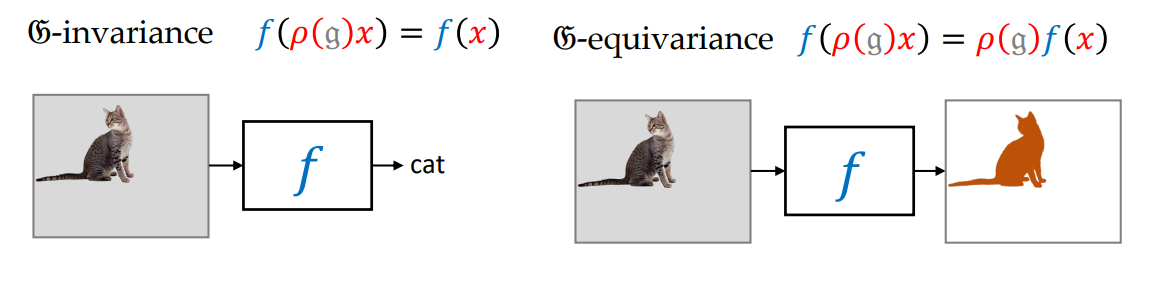
\includegraphics[width=1\linewidth]{Images/GDL/inva_equi.png}
    \caption{Hình ảnh minh họa về \textit{invariant} và \textit{equivariant}\cite{geometricdeep2022}}
\end{figure}

\section{Tensor field networks}
Tensor field networks (TFN) tác động trên các điểm với các đặc trưng liên quan. Một lớp \( \mathcal{L} \) lấy một tập hợp hữu hạn \( \mathcal{S} \) là các vector trong \( \mathbb{R}^3 \) và một vector trong \( \mathcal{X} \) tại mỗi điểm trong \( \mathcal{S} \) và đầu ra là một vector trong \( \mathcal{Y} \) tại mỗi điểm trong \( \mathcal{S} \), trong đó \( \mathcal{X} \) và \( \mathcal{Y} \) là các không gian vector\cite{thomas2018tensorfieldnetworksrotation}. Báo cáo viết điều này như sau

\[
\mathcal{L} (\vec{r}_a, x_a) = (\vec{r}_a, y_a)
\]

trong đó \( \vec{r}_a \in \mathbb{R}^3 \) là các tọa độ điểm và \( x_a \in \mathcal{X}, y_a \in \mathcal{Y} \) là các vector đặc trưng (với \( a \) là một chỉ mục trên các điểm trong \( \mathcal{S} \)). Sự kết hợp này của \( \mathbb{R}^3 \) với một không gian vector khác có thể được viết là \( \mathbb{R}^3 \oplus \mathcal{X} \), trong đó \( \oplus \) là phép nối (concatenation).

\subsection{Permutation equivariance}
$$\text{Điều kiện:} \hspace{0.5cm} \mathcal{L} \circ P_{\sigma} = P_{\sigma} \circ \mathcal{L}$$
Trong đó: $ P_{\sigma}(\vec{r}_a, x_a) := (\vec{r}_{\sigma(a)}, x_{\sigma(a)}) $ và $ \sigma$ là phép hoán vị các điểm mà các chỉ số tham chiếu đến.

\subsection{Translation equivariance}

$$\text{Điều kiện: } \mathcal{L} \circ \mathcal{T}_{\vec{t}} = \mathcal{T}_{\vec{t}} \circ \mathcal{L} $$

\text{trong đó } $\mathcal{T}_{\vec{t}}(\vec{r}_a, x_a) := (\vec{r}_a + \vec{t}, x_a)$. Điều kiện này tương tự như điều kiện tịnh tiến equivariance cho CNN.

% \text{Tất cả các tầng trong Phần 4 rõ ràng là equivariant tịnh tiến vì chúng ta chỉ sử dụng} \\
% \text{hiệu giữa hai điểm } $\vec{r}_i - \vec{r}_j$ \text{ (đối với các chỉ số } $i \text{ và } j$).

\subsection{Rotation equivariance}
Nhóm các phép quay 3D (thực) được gọi là $SO(3)$, một đa tạp có thể được tham số hóa bằng 3 số
(xem Goodman và Wallach\cite{goodman1998representations}). Cho $D^{\mathcal{X}}$ là một biểu diễn của $SO(3)$ trên không gian vectơ $\mathcal{X}$ (và $D^{\mathcal{Y}}$ trên $\mathcal{Y}$). Tác động với $g \in SO(3)$ trên $\vec{r} \in \mathbb{R}^3$ chúng ta viết là $R(g)\vec{r}$, và tác động trên $x \in \mathcal{X}$ cho kết quả là $D^{\mathcal{X}}(g)x$. 

Điều kiện: 
\begin{equation}\label{eq:1}
\centering
\mathcal{L} \circ \left[ R(g) \oplus D^{\mathcal{X}}(g) \right] = \left[ R(g) \oplus D^{\mathcal{Y}}(g) \right] \circ \mathcal{L}
\end{equation}

trong đó $\left[ R(g) \oplus D^{\mathcal{X}}(g) \right] (\vec{r}_a, x_a) = (R(g)\vec{r}_a, D^{\mathcal{X}}(g) x_a)$. (Đối với các layer trong bài báo này, chỉ có tác động
của $D^{\mathcal{Y}}(g)$ trên $\mathcal{Y}$ là không tầm thường, vì vậy chúng ta sẽ sử dụng quy ước bỏ qua đầu ra tầng $\mathbb{R}^3$ trong
các phương trình của chúng ta.) 

TFN đạt được tính equivariant với phép quay cục bộ bằng cách giới hạn các bộ lọc tích chập của chúng ta ở một dạng cụ thể. Các
đặc trưng có các loại khác nhau tương ứng với việc chúng biến đổi dưới dạng vô hướng, vectơ hoặc tenxơ bậc cao hơn\cite{thomas2018tensorfieldnetworksrotation}. 

TFN phân tích các biểu diễn thành các biểu diễn bất khả quy để đơn giản hóa phân tích của chúng ta. Các biểu diễn
bất khả quy của $SO(3)$ có kích thước $2l+1$ cho $l \in \mathbb{N}$ (bao gồm $l=0$) và là \textit{unitary}. Báo cáo sẽ sử dụng thuật ngữ “bậc quay” để chỉ $l$ trong biểu thức này. Các bậc quay $l=0, 1, 2$  tương ứng với vô hướng, vectơ trong không gian 3 chiều và ma trận đối xứng không dấu vết, tương ứng.

Các phần tử nhóm được biểu diễn bằng $D^{(l)}$, được gọi là \textit{ma trận Wigner-D} (xem Gilmore \cite{gilmore2008lie}); chúng ánh xạ các phần tử của $SO(3)$ thành ma trận $(2l+1) \times (2l+1)$ chiều. Đối với vô hướng và vectơ không gian 3 chiều, \textit{ma trận Wigner-D} (thực) là
$$
D^{(0)}(g) = 1 \quad \text{ và } \quad D^{(1)}(g) = R(g).
$$

\subsection{Cấu trúc của các lớp TFN}
Đầu vào và đầu ra của TFN là một tập hữu hạn $\mathcal{S}$ của các điểm trong $\mathbb{R}^3$ và một vector trong một biểu diễn của $SO(3)$ liên quan đến mỗi điểm\cite{thomas2018tensorfieldnetworksrotation}.

Chúng ta phân tích biểu diễn này thành các biểu diễn bất khả quy. Nói chung, có nhiều trường hợp của mỗi biểu diễn bất khả quy bậc quay $l$. Chúng tương tự với những gì thường được gọi là "độ sâu" của tích chập trong CNN tiêu chuẩn, vì vậy chúng ta sẽ đề cập đến những trường hợp khác nhau này là các kênh (channels). Chúng ta triển khai đối tượng này $V^{(l)}_{acm}$ như một từ điển với key $l$ (bậc quay) của các mảng đa chiều, mỗi mảng có hình dạng $[|S|, n_l, 2l + 1]$ (trong đó $n_l$ là số lượng kênh) tương ứng với [chỉ số điểm, chỉ số kênh, chỉ số biểu diễn]. Xem hình \ref{TFN_1} cho một ví dụ về cách mã hóa một hệ thống đơn giản trong ký hiệu này.

Báo cáo sẽ định nghĩa ba tầng TFN và chứng minh rằng chúng là equivariant. Tất cả những tầng này sẽ rõ ràng là invariant hoán vị và equivariant tịnh tiến, vì vậy để chứng minh rằng một tầng là equivariant, chúng ta chỉ cần chứng minh tính equivariant với phép quay cho một bậc quay tùy ý. Điều này yêu cầu cho thấy rằng khi đám mây điểm xoay và các đặc trưng đầu vào được biến đổi thành tenxơ, thì đầu ra đặc trưng cũng biến đổi thành tenxơ. 


% \begin{figure}[H]
%     \centering
%     \includegraphics[width=0.5\linewidth]{Images/TFN/image.png}
%     \caption{Ví dụ về $V^{(l)}_{acm}$ biểu diễn hai điểm khối lượng với vận tốc và gia tốc. Các dấu ngoặc vuông có màu cho biết các chỉ số $a$ (điểm), $c$ (kênh) và $m$ (biểu diễn). $(l)$ là khóa cho từ điển $V^{(l)}_{acm}$ của các tenxơ đặc trưng\cite{thomas2018tensorfieldnetworksrotation}.}
%     \label{TFN_1}
% \end{figure}

\subsubsection{Point convolution}
Lớp này là một thành phần cốt lõi của TFN. Tại mỗi lớp, đầu vào sẽ có cấu trúc là $V^{(l)}_{acm}$. Point convolution thực hiện phép toán giống nhau cho mỗi điểm $a$ và lấy mọi điểm còn lại như đầu vào. Ở đây, ta ký hiệu $\vec{r}$ là một vector trong không gian 3 chiều, $\hat{r}$ là vector $\vec{r}$ được chuẩn hóa có độ dài bằng 1 và $r$ là độ dài của $\vec{r}$. 

\paragraph{Spherical harmonics và filters}

Spherical harmonics $Y^{(l)}_m$ là các hàm từ các điểm trên một hình cầu đến các số phức hoặc số thực (trong đó $l$ là một số nguyên không âm và $m$ là bất kỳ số nguyên nào từ $-l$ đến $l$, bao gồm cả $-l$ và $l$). Spherical harmonics (thực) cho $l = 0$ (vô hướng) và $l = 1$ (vectơ không gian 3 chiều) là 
$$
Y^{(0)}(\hat{r}) \propto 1  \quad \text{và} \quad  Y^{(1)}(\hat{r}) \propto \hat{r}.
$$

Các hàm này equivariant với $SO(3)$; nghĩa là, với mọi $g \in SO(3)$ và $\hat{r}$, 
$$
Y^{(l)}_m (R(g) \hat{r}) = \sum_{m'} D^{(l)}_{mm'}(g) Y^{(l)}_{m'}(\hat{r}).
$$

Để thiết kế một phép tích chập điểm equivariant với phép quay, chúng ta muốn các bộ lọc equivariant với phép quay. Để các bộ lọc của chúng ta equivariant với phép quay, chúng ta giới hạn chúng ở dạng sau\cite{thomas2018tensorfieldnetworksrotation}:

\begin{equation}\label{eq:2}
F^{(l_f, l_i)}_{cm}(\hat{r}) = R^{(l_f, l_i)}_c (r) Y^{(l_f)}_m (\hat{r})  
\end{equation}

(trong đó $l_i$ và $l_f$ là các số nguyên không âm tương ứng với bậc quay của đầu vào và bộ lọc, tương ứng và $R^{(l_f, l_i)}_c : \mathbb{R}^{\ge 0} \rightarrow \mathbb{R}$ là các hàm được học, chứa hầu hết các tham số trong một TFN). Các bộ lọc có dạng này kế thừa thuộc tính biến đổi của các \textit{spherical harmonic} trong các phép quay vì $R(r)$ là một vô hướng trong $m$. Lựa chọn giới hạn bộ lọc này tương tự như việc sử dụng các \textit{circular harmonics} trong Worrall và các đồng nghiệp\cite{worrall2017harmonicnetworksdeeptranslation} (mặc dù chúng ta không có tương tự với độ lệch pha do tính không giao hoán của $SO(3)$). 

\paragraph{Kết hợp biểu diễn bằng tích tensor}

Bộ lọc và layer đầu vào đều kế thừa các biểu diễn của $SO(3)$ (nghĩa là, cả hai đều mang các chỉ số $l$ và $m$). Để tạo ra đầu ra mà chúng ta có thể đưa vào các tầng phía sau, chúng ta cần kết hợp đầu vào tầng và bộ lọc theo cách mà đầu ra cũng biến đổi một cách thích hợp (bằng cách kế thừa biểu diễn của $SO(3)$)\cite{thomas2018tensorfieldnetworksrotation}. 

Tích tenxơ của các biểu diễn là một quy tắc để kết hợp hai biểu diễn $D^{\mathcal{X}}$ và $D^{\mathcal{Y}}$ để nhận được một biểu diễn khác $D^{\mathcal{X}} \otimes D^{\mathcal{Y}}$ trên không gian vectơ $\mathcal{X} \otimes \mathcal{Y}$. Thuộc tính quan trọng của tích tenxơ là nó equivariant:
$$
D^{\mathcal{X}} \otimes D^{\mathcal{Y}} = D^{\mathcal{X} \otimes \mathcal{Y}}
$$

Bây giờ hãy xem xét tích tenxơ của hai biểu diễn có bậc $l_1$ và $l_2$ (trong đó chúng ta sử dụng quy ước ký hiệu thông thường là chỉ sử dụng $l$ để chỉ không gian vectơ $(2l + 1)$ chiều biểu diễn bậc quay $l$). Đối với các biểu diễn không thể rút gọn với $u^{(l_1)} \in l_1$ và $v^{(l_2)} \in l_2$, $(u^{(l_1)} \otimes v^{(l_2)}) \in l_1 \otimes l_2$ có thể được tính bằng cách sử dụng các hệ số Clebsch–Gordan (xem Griffiths \cite{Griffiths_Schroeter_2018}) (ký hiệu là $C$):
$$
(u \otimes v)^{(l)}_m = \sum_{m_1 = -l_1}^{l_1} \sum_{m_2 = -l_2}^{l_2} C^{ (l, m)}_{(l_1, m_1),(l_2, m_2)} u^{(l_1)}_{m_1} v^{(l_2)}_{m_2}
$$

Tích tenxơ này tạo ra các giá trị khác không chỉ cho $l$ nằm trong khoảng từ $|l_1 - l_2|$ đến $(l_1 + l_2)$ (bao gồm cả $|l_1 - l_2|$ và $(l_1 + l_2)$) ($m$ là bất kỳ số nguyên nào từ $-l$ đến $l$, bao gồm cả $-l$ và $l$). Các hệ số Clebsch–Gordan (thực) cho $l = 0$ và $l = 1$ chỉ là những cách quen thuộc để kết hợp các vô hướng và vectơ: Đối với $1 \otimes 1 \rightarrow 0$ và $1 \otimes 1 \rightarrow 1$, 
$$
C^{ (0, 0)}_{(1, i),(1, j)} \propto \delta_{ij}  \quad \quad  C^{ (1, i)}_{(1, j),(1, k)} \propto \epsilon_{ijk}
$$
đó là tích vô hướng và tích có hướng cho các vectơ 3D, tương ứng. Trường hợp $0 \otimes 0 \rightarrow 0$ chỉ là phép nhân thông thường của hai vô hướng và $0 \otimes 1 \rightarrow 1$ và $1 \otimes 0 \rightarrow 1$ tương ứng với phép nhân vô hướng của một vectơ. 

\subsubsection{Định nghĩa cấu trúc của layer}

Một đầu vào cho trước sẽ kế thừa một biểu diễn, một bộ lọc sẽ kế thừa một biểu diễn khác và cùng nhau chúng tạo ra đầu ra ở nhiều bậc quay có thể\cite{thomas2018tensorfieldnetworksrotation} . Chúng ta có thể kết hợp mọi thứ lại với nhau trong định nghĩa tầng tích chập theo điểm của chúng ta:

\begin{equation}\label{eq:3}
\mathcal{L}^{(l_o)}_{acm_o} (\vec{r}_a, V^{(l_i)}_{acm_i})  :=  \sum_{m_f, m_i}  C^{(l_o, m_o)}_{(l_f, m_f),(l_i, m_i)} \sum_{b \in \mathcal{S}} F^{(l_f, l_i)}_{cm_f}(\vec{r}_{ab}) V^{(l_i)}_{bcm_i}
\end{equation}

(trong đó $\vec{r}_{ab} := \vec{r}_a - \vec{r}_b$ và các chỉ số $i$, $f$ và $o$ biểu thị cho các biểu diễn của đầu vào, bộ lọc và đầu ra, tương ứng). Một phép tích chập điểm của một bộ lọc $l_f$ trên một đầu vào $l_i$ mang lại đầu ra ở $2\text{min}(l_i, l_f) + 1$ bậc quay $l_o$ khác nhau (một cho mỗi số nguyên từ $|l_i - l_f|$ đến $(l_i + l_f)$, bao gồm cả $|l_i - l_f|$ và $(l_i + l_f)$), mặc dù khi thiết kế một mạng cụ thể, chúng ta có thể chọn không tính toán hoặc sử dụng một số đầu ra đó\cite{thomas2018tensorfieldnetworksrotation}.

Tính equivariant của bộ lọc $F$ (phương trình \ref{eq:2}) và tính equivariant của các hệ số Clebsch–Gordan cùng ngụ ý rằng các phép tích chập điểm là equivariant.

\subsubsection{Self-interaction}
Báo cáo làm theo Schütt et al. \cite{schütt2017schnetcontinuousfilterconvolutionalneural} trong việc sử dụng các phép tích chập điểm để chia tỷ lệ các vectơ đặc trưng theo từng phần tử và sử dụng các lớp \textit{Self-interaction} để trộn các thành phần của vectơ đặc trưng tại mỗi điểm. Các layer \textit{Self-interaction} tương tự như các tích chập 1x1 và chúng hoạt động giống như các bộ lọc $l = 0$ (vô hướng):

$$
\sum_{c'} W^{(l)}_{cc'} V^{(l)}_{ac'm}
$$

Nói chung, mỗi bậc quay có trọng số khác nhau vì có thể có số lượng kênh khác nhau tương ứng với bậc quay đó. Tuy nhiên, cùng một trọng số được sử dụng cho mọi $m$ cho một bậc cho trước; điều này rất cần thiết để duy trì tính equivariant. Đối với $l = 0$, chúng ta cũng có thể sử dụng độ lệch.

Các ma trận $D$ giao hoán với ma trận trọng số $W$ vì $W$ không có chỉ số biểu diễn $m$, vì vậy tầng này là equivariant với $l > 0$. Tính equivariant với $l = 0$ là đơn giản vì $D^{(0)} = 1$. 

\subsubsection{Nonlinearity}
Lớp phi tuyến (\textit{nonlinearity}) hoạt động như một phép biến đổi vô hướng trong không gian $l$ (nghĩa là, dọc theo chiều $m$). Đối với các kênh $l = 0$, chúng ta có thể sử dụng 
$$
\eta^{(0)}(V^{(0)}_{ac} + b^{(0)}_c) \quad \text{và} \quad \eta^{(l)}(\| V \|_{ac}^{(l)} + b^{(l)}_c)V^{(l)}_{acm} \quad \text{trong đó} \quad \| V \|_{ac}^{(l)} := \sqrt{\sum_m | V^{(l)}_{acm}|^2} 
$$ 
cho một số hàm $\eta^{(l)}: \mathbb{R} \rightarrow \mathbb{R}$ (có thể khác nhau cho mỗi $l$) và độ lệch $b^{(l)}_c$. Lưu ý rằng 
$$
\| D(g) V \| = \| V \|
$$
vì $D$ là một biểu diễn đơn vị. Do đó, tầng này là một phép biến đổi vô hướng trong chỉ số biểu diễn $m$, vì vậy nó equivariant. 